\documentclass[handout, notes=hide]{beamer}

\usepackage{amsmath}
\usepackage{yhmath}
\usepackage{eqnarray}
\usepackage{attrib}
\graphicspath{{./figures/}}
\DeclareGraphicsExtensions{.pdf,.jpeg,.png,.jpg}
\usepackage[export]{adjustbox}
\usepackage{framed}
\usepackage{tikz}
\usepackage{listings}
\usepackage{color}

\usetheme{Rochester}
\usecolortheme{beaver}

\setbeamertemplate{bibliography entry title}{}
\setbeamertemplate{bibliography entry location}{}
\setbeamertemplate{bibliography entry note}{}

\renewcommand{\thefootnote}{\fnsymbol{footnote}}
\newcommand{\prescite}[1]{\footnote{\cite{#1}}}
\newcommand{\prestext}[1]{\footnotetext{\cite{#1}}}
\newcommand{\emaillink}[1]{\href{mailto:#1}{\nolinkurl{#1}}}
\usepackage{perpage}
\MakePerPage{footnote}

\definecolor{shadecolor}{HTML}{E8F8FF}

\def\etal{{\it et al.}}
\def\etc{{\it etc.}}
\def\eg{{\it e.g.}}
\def\ie{{\it i.e.}}
\def\cf{{\it cf.}}
\def\qv{{\it q.v.}}
\def\qqv{{\it qq.v.}}
\def\st{s.t.\ }
\def\concat{\mathbin{|}}

\newtheorem{claimnum}{Claim}
\newtheorem{question}{Question}[section]

\newcommand\Wider[2][3em]{\makebox[\linewidth][c]{\begin{minipage}{\dimexpr\textwidth+#1\relax}\raggedright#2\end{minipage}}}
\newcolumntype{Y}{>{\centering\arraybackslash}X}
\newcommand{\comment}[1]{\marginnote{\textit{\textbf{\scriptsize{#1}}}}}
\newcolumntype{e}{@{\qquad}}



\definecolor{mygreen}{rgb}{0,0.6,0}
\definecolor{mygray}{rgb}{0.5,0.5,0.5}
\definecolor{mymauve}{rgb}{0.58,0,0.82}
 
%Customize a bit the look
\lstset{ %
	backgroundcolor=\color{white}, % choose the background color; you must add \usepackage{color} or \usepackage{xcolor}
	basicstyle=\fontsize{6pt}{6}, % the size of the fonts that are used for the code
	breakatwhitespace=false, % sets if automatic breaks should only happen at whitespace
	breaklines=true, % sets automatic line breaking
	captionpos=, % sets the caption-position to bottom
	commentstyle=\color{mygreen}, % comment style
	deletekeywords={...}, % if you want to delete keywords from the given language
	escapeinside={\%*}{*)}, % if you want to add LaTeX within your code
	extendedchars=true, % lets you use non-ASCII characters; for 8-bits encodings only, does not work with UTF-8
	frame=single, % adds a frame around the code
	keepspaces=true, % keeps spaces in text, useful for keeping indentation of code (possibly needs columns=flexible)
	keywordstyle=\color{blue}, % keyword style
	% language=Octave, % the language of the code
	morekeywords={*,...}, % if you want to add more keywords to the set
	numbers=left, % where to put the line-numbers; possible values are (none, left, right)
	numbersep=5pt, % how far the line-numbers are from the code
	numberstyle=\tiny\color{mygray}, % the style that is used for the line-numbers
	rulecolor=\color{black}, % if not set, the frame-color may be changed on line-breaks within not-black text (e.g. comments (green here))
	showspaces=false, % show spaces everywhere adding particular underscores; it overrides 'showstringspaces'
	showstringspaces=false, % underline spaces within strings only
	showtabs=false, % show tabs within strings adding particular underscores
	stepnumber=1, % the step between two line-numbers. If it's 1, each line will be numbered
	stringstyle=\color{mymauve}, % string literal style
	tabsize=2, % sets default tabsize to 2 spaces
	title=\lstname % show the filename of files included with \lstinputlisting; also try caption instead of title
}
%END of listing package%
 
\definecolor{darkgray}{rgb}{.4,.4,.4}
\definecolor{purple}{rgb}{0.65, 0.12, 0.82}
 
%define Javascript language
\lstdefinelanguage{JavaScript}{
	keywords={typeof, new, true, false, catch, function, return, null, catch, switch, var, if, in, while, do, else, case, break},
	keywordstyle=\color{blue}\bfseries,
	ndkeywords={class, export, boolean, throw, implements, import, this},
	ndkeywordstyle=\color{darkgray}\bfseries,
	identifierstyle=\color{black},
	sensitive=false,
	comment=[l]{//},
	morecomment=[s]{/*}{*/},
	commentstyle=\color{purple}\ttfamily,
	stringstyle=\color{red}\ttfamily,
	morestring=[b]',
	morestring=[b]"
}
 
\lstset{
	language=JavaScript,
	extendedchars=true,
	basicstyle=\fontsize{6pt}{6}\ttfamily,
	showstringspaces=false,
	showspaces=false,
	numbers=left,
	numberstyle=\fontsize{6pt}{6},
	numbersep=6pt,
	tabsize=2,
	breaklines=true,
	showtabs=false,
	captionpos=
}

%%%%%%%%%%%%%%%%%%%%%%%%%%%%%%%%%%%%%%%%%%%%%%%%%%%%%%%%%%%%%%%%%%%%%%%%%%%%%%%%%%

\begin{document}

\title{Cracking PwdHash: A Bruteforce Attack on Client-side Password Hashing}
\subtitle{Passwords 2016}
\author{David Llewellyn-Jones, Graham Rymer\\\vspace{0.5cm}\scriptsize\{David.Llewellyn-Jones, Graham.Rymer\}@cl.cam.ac.uk}
\institute{University of Cambridge}
\date{7th December 2016}

%%%%%%%%%%%%%%%%%%%%%%%%%%%%%%%%%%%%%%%%%

\renewcommand{\thefootnote}{\arabic{footnote}}

\frame{
\titlepage
\begin{tikzpicture}[remember picture,overlay]
\node[anchor=north east,yshift=-4pt,xshift=-4pt] at (current page.north east) {\includegraphics[height=0.9cm]{ucam-logo-colour}};
\end{tikzpicture}
}
\note{
\setlength{\parskip}{0.5em}
It begins.
}

\renewcommand{\thefootnote}{\fnsymbol{footnote}}

%%%%%%%%%%%%%%%%%%%%%%%%%%%%%%%%%%%%%%%%%

\begin{frame}
\frametitle{PwdHash}
\framesubtitle{What is PwdHash}
\setlength{\parskip}{0.5em}

\begin{columns}[T]
\begin{column}[T]{1.15\textwidth}
\vspace{-0.cm}
\hspace{-0.0cm}
\includegraphics[width=1.0\textwidth]{pwdhashsite}
\end{column}
\end{columns}

\end{frame}
\note{
\setlength{\parskip}{0.5em}
\begin{enumerate}
\item A password generating tool.
\item The user provides a site and a master password.
\item PwdHash generates a unique password for the site using a one-way hash function.
\end{enumerate}
}


%%%%%%%%%%%%%%%%%%%%%%%%%%%%%%%%%%%%%%%%%

\begin{frame}
\frametitle{PwdHash}
\framesubtitle{Where did PwdHash come from}
\setlength{\parskip}{0.5em}

\begin{columns}[T]
\begin{column}[T]{1.315\textwidth}
\vspace{-0.8cm}
\hspace{-0.8cm}
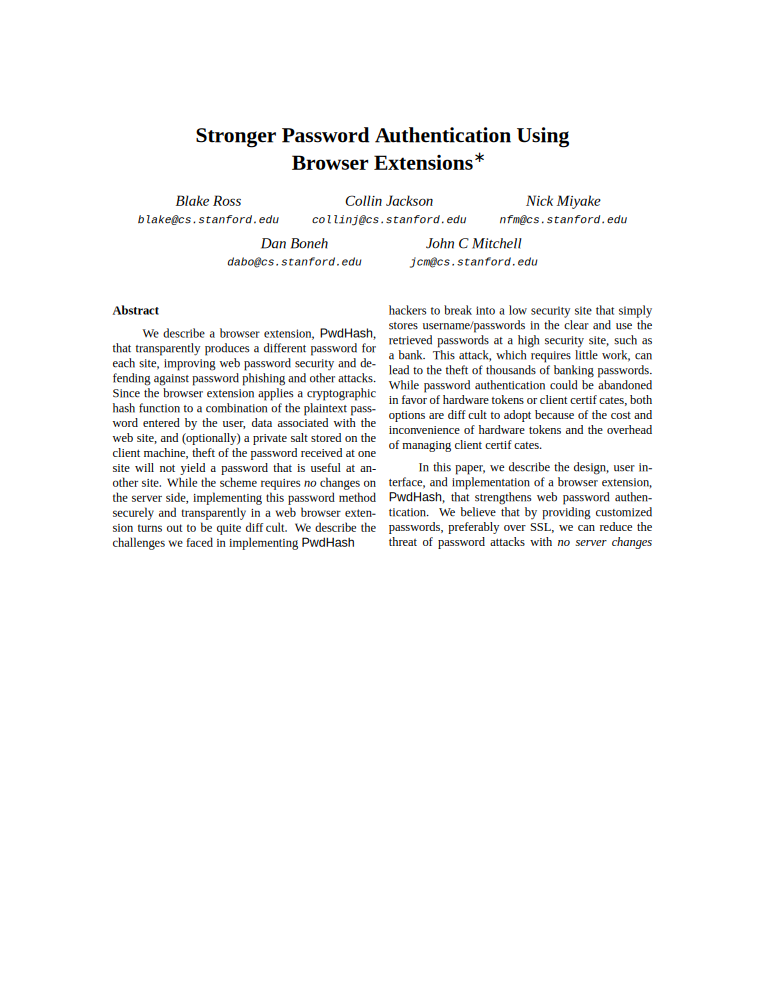
\includegraphics[width=1.0\textwidth]{ross2005}
\end{column}
\end{columns}

\end{frame}
\note{
\setlength{\parskip}{0.5em}
\begin{enumerate}
\item Published at USENIX 2005.
\item Authored by Blake Ross, Collin Jackson, Nick Mayake, Dan Boneh and John C Mitchell.
\item At the time at Stanford, but now in various places.
\begin{enumerate}
\item Blake co-founded Mozilla, until recently Director of Product at Facebook.
\item Jackson founded Apportable for cross-platform app development.
\item Miyake was a student at the time.
\item Dan Boneh is Professor of Computer Science and Electrical Engineering at Stanford.
\item John C Mitchell is Professor of Computer Science and Electrical Engineering at Stanford.
\end{enumerate}
\end{enumerate}
}

%%%%%%%%%%%%%%%%%%%%%%%%%%%%%%%%%%%%%%%%%

\begin{frame}
\frametitle{Client-Side Hashing}
\framesubtitle{Not the first, or last}
\setlength{\parskip}{0.5em}

\begin{columns}[T]
\begin{column}[T]{0.6\textwidth}
\setlength{\parskip}{0.5em}
There are other examples of client-side hashing techniques
\begin{enumerate}
\item Passpet
\item PwdHash++
\item RndPhrase
\end{enumerate}
\end{column}
\begin{column}[T]{0.4\textwidth}
\vspace{0.0em}
\includegraphics[width=1.0\textwidth]{android}
\end{column}
\end{columns}


\end{frame}
\note{
\setlength{\parskip}{0.5em}
\begin{enumerate}
\item Android app by Philipp Wolfer, updated April 2015 \url{https://play.google.com/store/apps/details?id=com.uploadedlobster.PwdHash}.
\item Firefox plugin updated February 2016 \url{https://addons.mozilla.org/en-US/firefox/addon/pwdhash/}
\item PwdHash generates a unique password for the site using a one-way hash function.
\end{enumerate}
}

%%%%%%%%%%%%%%%%%%%%%%%%%%%%%%%%%%%%%%%%%

\begin{frame}
\frametitle{PwdHash Operation}
\framesubtitle{How does it work?}
\setlength{\parskip}{0.5em}

\begin{columns}[T]
\begin{column}[T]{1.1\textwidth}
\vspace{0.0em}
\includegraphics[width=1.0\textwidth]{process01}
\end{column}
\end{columns}


\end{frame}
\note{
\setlength{\parskip}{0.5em}
}

%%%%%%%%%%%%%%%%%%%%%%%%%%%%%%%%%%%%%%%%%

\begin{frame}
\frametitle{PwdHash Operation}
\framesubtitle{How does it work?}
\setlength{\parskip}{0.5em}

\begin{columns}[T]
\begin{column}[T]{1.1\textwidth}
\vspace{0.0em}
\includegraphics[width=1.0\textwidth]{process02}
\end{column}
\end{columns}


\end{frame}
\note{
\setlength{\parskip}{0.5em}
}

%%%%%%%%%%%%%%%%%%%%%%%%%%%%%%%%%%%%%%%%%

\begin{frame}
\frametitle{PwdHash Operation}
\framesubtitle{How does it work?}
\setlength{\parskip}{0.5em}

\begin{columns}[T]
\begin{column}[T]{1.1\textwidth}
\vspace{0.0em}
\includegraphics[width=1.0\textwidth]{process03}
\end{column}
\end{columns}


\end{frame}
\note{
\setlength{\parskip}{0.5em}
}

%%%%%%%%%%%%%%%%%%%%%%%%%%%%%%%%%%%%%%%%%

\begin{frame}
\frametitle{PwdHash Operation}
\framesubtitle{How does it work?}
\setlength{\parskip}{0.5em}

\begin{columns}[T]
\begin{column}[T]{1.1\textwidth}
\vspace{0.0em}
\includegraphics[width=1.0\textwidth]{process04}
\end{column}
\end{columns}


\end{frame}
\note{
\setlength{\parskip}{0.5em}
}

%%%%%%%%%%%%%%%%%%%%%%%%%%%%%%%%%%%%%%%%%

\begin{frame}
\frametitle{Perceived Benefits}
\framesubtitle{What makes a good password?}
\setlength{\parskip}{0.5em}

\vspace{+2.0em}

\begin{columns}[T]
\begin{column}[T]{0.6\textwidth}
\setlength{\parskip}{0.5em}

Unique to each site.

Contains complex mix of characters.

Contains at least $n$ characters.

Easy for the owner to remember, hard for anyone else to guess.

\end{column}
\begin{column}[T]{0.4\textwidth}
\vspace{-3.0em}
\hspace{-7.0em}
\includegraphics[width=1.6\textwidth]{rockyou}
\end{column}
\end{columns}

\end{frame}
\note{
\setlength{\parskip}{0.5em}
}

%%%%%%%%%%%%%%%%%%%%%%%%%%%%%%%%%%%%%%%%%

\begin{frame}
\frametitle{Other Benefits}
\framesubtitle{}
\setlength{\parskip}{0.5em}

\begin{columns}[T]
\begin{column}[T]{0.5\textwidth}
\setlength{\parskip}{0.5em}

No database of passwords.

Can be used anywhere.

Integrates into the browser.

Protects against phishing.

Can tailor the output to suit site restrictions.

\end{column}
\begin{column}[T]{0.5\textwidth}
\includegraphics[width=1.0\textwidth]{plugin}
\end{column}
\end{columns}

\end{frame}
\note{
\setlength{\parskip}{0.5em}
}

%%%%%%%%%%%%%%%%%%%%%%%%%%%%%%%%%%%%%%%%%

\begin{frame}
\frametitle{The Detail}
\framesubtitle{How does PwdHash work?}
\setlength{\parskip}{0.5em}

\begin{columns}[T]
\begin{column}[T]{1.0\textwidth}

\lstinputlisting[language=Javascript]{figures/pwdhashcode.js}

\end{column}
\end{columns}


\end{frame}
\note{
\setlength{\parskip}{0.5em}
\begin{enumerate}
\item HMAC-MD5 is 16-types long.
\item Amounts to 22 characters in base64.
\item Passwords over 22 characters have A or zero byte repeatedly added, then no rotation.
\end{enumerate}
}

%%%%%%%%%%%%%%%%%%%%%%%%%%%%%%%%%%%%%%%%%

\begin{frame}
\frametitle{Example Output}
\framesubtitle{}
\setlength{\parskip}{0.5em}

\begin{columns}[T]
\begin{column}[T]{1.0\textwidth}
\setlength{\parskip}{0.5em}

\renewcommand{\arraystretch}{1.5}
\begin{tabular}{l|l|l}
{\bf Password} & {\bf Site} & {\bf PwdHash password} \\ \hline
passwords2016.rub.de & password & KC3n2GBOg6 \\
passwords2016.rub.de & password? & VRGyE+5B0Ws \\
linkedin.com & password & WmPLC7OyIq \\
linkedin.com & password012345 & QDHU4ZGr7dNfZOym \\
\end{tabular}
\end{column}
\end{columns}

\end{frame}
\note{
\setlength{\parskip}{0.5em}
}

%%%%%%%%%%%%%%%%%%%%%%%%%%%%%%%%%%%%%%%%%

\begin{frame}
\frametitle{The Problem}
\framesubtitle{Leaky password databases}
\setlength{\parskip}{0.5em}

\begin{columns}[T]
\begin{column}[T]{0.6\textwidth}
\setlength{\parskip}{0.5em}

HIBP contains 1.3 billion compromised accounts

@dumpmon identifies 46 significant database dumps per day

Discovered 1 million unique hashes in 12 months to May 2015

\end{column}
\begin{column}[T]{0.4\textwidth}
\vspace{0.0em}
\includegraphics[width=1.0\textwidth]{hibp}
\end{column}
\end{columns}


\end{frame}
\note{
\setlength{\parskip}{0.5em}
\begin{enumerate}
\item ??
\end{enumerate}
}

%%%%%%%%%%%%%%%%%%%%%%%%%%%%%%%%%%%%%%%%%

\begin{frame}
\frametitle{Salting and Hashing}
\framesubtitle{Modern best practice}
\setlength{\parskip}{0.5em}

\begin{columns}[T]
\begin{column}[T]{1.0\textwidth}
\setlength{\parskip}{0.5em}

Don't store the password in plaintext.

Store a salted, hashed version:

$$
V = S \concat H(P \concat S)
$$

$V$ is the stored value,

$S$ a random salt,

$P$ the password,

$H$ is a one-way hash function.

\end{column}
\end{columns}


\end{frame}
\note{
\setlength{\parskip}{0.5em}
\begin{enumerate}
\item LinkedIn used unsalted SHA1.
\item Yahoo (late 2014, 500 million compromised accounts), mostly bcrypt hashed.
\end{enumerate}
}

%%%%%%%%%%%%%%%%%%%%%%%%%%%%%%%%%%%%%%%%%

\begin{frame}
\frametitle{Password Recovery}
\framesubtitle{Reversing salted hashes}
\setlength{\parskip}{0.5em}

\begin{columns}[T]
\begin{column}[T]{1.0\textwidth}
\setlength{\parskip}{0.5em}
Salting prevents use of rainbow tables.

Hashes must be reversed by generating the hash and comparing.

Recovery tools have responded by utilising GPUs.

GPUs aren't necessarily as fast as CPUs, but are highly parallelisable.

\end{column}
\end{columns}


\end{frame}
\note{
\setlength{\parskip}{0.5em}
\begin{enumerate}
\item ??
\end{enumerate}
}

%%%%%%%%%%%%%%%%%%%%%%%%%%%%%%%%%%%%%%%%%

\begin{frame}
\frametitle{Stats}
\framesubtitle{Password recovery is {\it fast}}
\setlength{\parskip}{0.5em}

\begin{columns}[T]
\begin{column}[T]{0.6\textwidth}
\setlength{\parskip}{0.5em}
Ruddick and Yan, 2016, analysed oclHashcat
\begin{itemize}
\item Radeon HD6870, 1120 processor streams at 900 MHz
\item SHA1, 1462 MH/s
\end{itemize}

Jeremy Gosney, Sagitta

\begin{itemize}
\item $8 \times$ Nvidia GTX Titan X
\item SHA1, 48.87 GH/s
\item bcrypt (cost 5) 133 KH/s.
\end{itemize}


\end{column}
\begin{column}[T]{0.4\textwidth}
\vspace{0.0em}
\includegraphics[width=1.0\textwidth]{hashcat}
\end{column}
\end{columns}


\end{frame}
\note{
\setlength{\parskip}{0.5em}
\begin{enumerate}
\item For SHA1, a 12-character base64 password space can be exhausted in just over 12 hours.
\end{enumerate}
}

%%%%%%%%%%%%%%%%%%%%%%%%%%%%%%%%%%%%%%%%%

\begin{frame}
\frametitle{Refining the Space}
\framesubtitle{Not just brute force}
\setlength{\parskip}{0.5em}

\begin{columns}[T]
\begin{column}[T]{1.0\textwidth}
\setlength{\parskip}{0.5em}

Scanning entire password space still not tractable.

Use dictionaries and rules to refine.

\begin{enumerate}
\item Masks
\item Combinator
\item Hybrid
\item Rule-based
\end{enumerate}

Generated PwdHash passwords aren't susceptible to these attacks.


\end{column}
\end{columns}


\end{frame}
\note{
\setlength{\parskip}{0.5em}
\begin{enumerate}
\item Uniform distribution of characters.
\item Would require complete coverage of the password space.
\item The master password, however, is susceptible.
\end{enumerate}
}

%%%%%%%%%%%%%%%%%%%%%%%%%%%%%%%%%%%%%%%%%

\begin{frame}
\frametitle{PwdHash Attack}
\framesubtitle{Add the PwdHash hash into the hashcat process}
\setlength{\parskip}{0.5em}

\includegraphics[width=0.8\textwidth]{hashcat-usual}

\end{frame}
\note{
\setlength{\parskip}{0.5em}
\begin{enumerate}
\item ??
\end{enumerate}
}

%%%%%%%%%%%%%%%%%%%%%%%%%%%%%%%%%%%%%%%%%

\begin{frame}
\frametitle{PwdHash Attack}
\framesubtitle{Add the PwdHash hash into the hashcat process}
\setlength{\parskip}{0.5em}

\includegraphics[width=0.8\textwidth]{hashcat-pwdhash}

\end{frame}
\note{
\setlength{\parskip}{0.5em}
\begin{enumerate}
\item ??
\end{enumerate}
}


%%%%%%%%%%%%%%%%%%%%%%%%%%%%%%%%%%%%%%%%%

\begin{frame}
\frametitle{Hashcat Optimisations}
\framesubtitle{}
\setlength{\parskip}{0.5em}

\begin{columns}[T]
\begin{column}[T]{1.0\textwidth}
\setlength{\parskip}{0.5em}

Hashcat performs a variety of clever optimisations.

Can't just add the PwdHash straight in.

\end{column}
\end{columns}


\end{frame}
\note{
\setlength{\parskip}{0.5em}
\begin{enumerate}
\item A password generating tool.
\item The user provides a site and a master password.
\item PwdHash generates a unique password for the site using a one-way hash function.
\end{enumerate}
}

%%%%%%%%%%%%%%%%%%%%%%%%%%%%%%%%%%%%%%%%%

\begin{frame}
\frametitle{PwdHash Attack}
\framesubtitle{Add the PwdHash hash into the hashcat process}
\setlength{\parskip}{0.5em}

\includegraphics[width=1.0\textwidth]{process-orig}

\end{frame}
\note{
\setlength{\parskip}{0.5em}
\begin{enumerate}
\item ??
\end{enumerate}
}

%%%%%%%%%%%%%%%%%%%%%%%%%%%%%%%%%%%%%%%%%

\begin{frame}
\frametitle{PwdHash Attack}
\framesubtitle{Add the PwdHash hash into the hashcat process}
\setlength{\parskip}{0.5em}

\includegraphics[width=1.0\textwidth]{process-mangle}

\end{frame}
\note{
\setlength{\parskip}{0.5em}
\begin{enumerate}
\item ??
\end{enumerate}
}

%%%%%%%%%%%%%%%%%%%%%%%%%%%%%%%%%%%%%%%%%

\begin{frame}
\frametitle{Results}
\framesubtitle{Summary of leaked hash databases tested}
\setlength{\parskip}{0.5em}

\begin{columns}[T]
\begin{column}[T]{1.0\textwidth}
\setlength{\parskip}{0.5em}

\fontsize{9pt}{14}\selectfont

\begin{tabular}{l|p{2.0cm}|p{2.0cm}|p{2.2cm}}
	{\bf Domain} & Stratfor.com & Rootkit.com  & Linkedin.com \\ \hline
	{\bf Year of leak}   & 2011         & 2011         & 2012 \\
	{\bf Hashes} & 822 657      & 58 677       & 2936840/ 6458020 \\
	{\bf Type}   & Unsalted MD5 & Unsalted MD5 & Unsalted SHA1 \\
	{\bf Attribution} & ``Anonymous'' & ``Anonymous'' & Unknown \\
	{\bf Previous best effort} & 93\% & 95\% & 77\% \\
	{\bf Cracking speed} & 42008.5 kH/s & 42193.8 kH/s & 39762.2 kH/s \\
	{\bf } & (11.40ms/H) & (11.35ms/H) & (14.88ms/H) \\
	{\bf Cracking time} & 27s & 27s & 28s \\
	{\bf Passwords recovered} & 1 & 3 & 75 \\
\end{tabular}

\end{column}
\end{columns}


\end{frame}
\note{
\setlength{\parskip}{0.5em}
\begin{enumerate}
\item ??
\end{enumerate}
}

%%%%%%%%%%%%%%%%%%%%%%%%%%%%%%%%%%%%%%%%%

\begin{frame}
\frametitle{Benchmarks}
\framesubtitle{Testing rig}
\setlength{\parskip}{0.5em}

\begin{columns}[T]
\begin{column}[T]{0.7\textwidth}
\setlength{\parskip}{0.5em}

Amazon EC2 g2.2xlarge instance

Eight Intel Xeon E5-2670 vCPUs - 2.60GHz

NVIDIA GRID K520 - 800 MHz

Two GPUs with 1536 CUDA cores (3072 total)

4GB of graphics memory and 8 GB main RAM

Costs \$0.65 per hour

\end{column}
\begin{column}[T]{0.3\textwidth}
\vspace{0.0em}
\includegraphics[width=1.0\textwidth]{k520}
\end{column}
\end{columns}

\end{frame}
\note{
\setlength{\parskip}{0.5em}
\begin{enumerate}
\item ??
\end{enumerate}
}

%%%%%%%%%%%%%%%%%%%%%%%%%%%%%%%%%%%%%%%%%

\begin{frame}
\frametitle{Benchmarks}
\framesubtitle{How does this impact performance?}
\setlength{\parskip}{0.5em}

\includegraphics[width=1.0\textwidth]{benchmarks}

\end{frame}
\note{
\setlength{\parskip}{0.5em}
\begin{enumerate}
\item ??
\end{enumerate}
}

%%%%%%%%%%%%%%%%%%%%%%%%%%%%%%%%%%%%%%%%%

\begin{frame}
\frametitle{Benchmarks}
\framesubtitle{How does this impact performance?}
\setlength{\parskip}{0.5em}

\begin{columns}[T]
\begin{column}[T]{1.0\textwidth}

\fontsize{9pt}{14}\selectfont

\begin{tabular}{p{4cm}|p{2.8cm}|p{2.8cm}}
	{\bf Hash type} & {\bf Speed (MH/s)} & {\bf Overhead (factor)} \\ \hline
	MD5 & 2316.7 & 1.0 \\
	MD5 PwdHash & 2410.7 & 0.961 \\
	SHA1 & 616.9 & 1.0 \\
	SHA1 PwdHash & 645.1 & 0.956 \\
	HMAC-MD5 & 780.3 & 1.0 \\
	HMAC-MD5 PwdHash & 76.9527 & 10.140 \\
	Stratfor.com MD5 & 42.0085 & n/a \\
	Rootkit.com MD5 & 42.1938 & n/a \\
	Linkedin.com SHA1 & 39.7622 & n/a \\
\end{tabular}%

\end{column}
\end{columns}

\end{frame}
\note{
\setlength{\parskip}{0.5em}
\begin{enumerate}
\item ??
\end{enumerate}
}

%%%%%%%%%%%%%%%%%%%%%%%%%%%%%%%%%%%%%%%%%

\begin{frame}
\frametitle{Results}
\framesubtitle{Master passwords}
\setlength{\parskip}{0.5em}

\begin{columns}[T]
\begin{column}[T]{1.0\textwidth}
\setlength{\parskip}{0.5em}

\fontsize{8pt}{15}\selectfont

\begin{tabular}{p{1.8cm}|p{6cm}|p{1.8cm}}
	{\bf Domain} & {\bf Leaked hash} & {\bf Password} \\ \hline
	Stratfor & {\tt e9c0873319ec03157f3fbc81566ddaa5} & frogdog \\
	Rootkit & {\tt 2261bac1dfe3edeac939552c0ca88f35} & zugang \\
	Rootkit & {\tt 43679e624737a28e9093e33934c7440d} & ub2357 \\
	Rootkit & {\tt dd70307400e1c910c714c66cda138434} & erpland \\
	LinkedIn & {\tt 508c2195f51a6e70ce33c2919531909736426c6a} & 5tgb6yhn \\
	LinkedIn & {\tt ed92efc65521fe5074d65897da554d0a629f9dc7} & Superman1938 \\
	LinkedIn & {\tt 5a9e7cc189fa6cf1dac2489c5b81c28a3eca8b72} & Fru1tc4k3 \\
	LinkedIn & {\tt ba1c6d86860c1b0fa552cdb9602fdc9440d912d4} & meideprac01 \\
	LinkedIn & {\tt fd08064094c29979ce0e1c751b090adaab1f7c34} & jose0849 \\
	LinkedIn & {\tt 5264d95e1dd41fcc1b60841dd3d9a37689e217f7} & linkedin
\end{tabular}

\end{column}
\end{columns}


\end{frame}
\note{
\setlength{\parskip}{0.5em}
\begin{enumerate}
\item ??
\end{enumerate}
}

%%%%%%%%%%%%%%%%%%%%%%%%%%%%%%%%%%%%%%%%%

\begin{frame}
\frametitle{Mitigation}
\framesubtitle{Fixing PwdHash}
\setlength{\parskip}{0.5em}

\begin{columns}[T]
\begin{column}[T]{0.6\textwidth}
\setlength{\parskip}{0.5em}

Use slow hashing algorithm.

Include the client salt.

Fix hash overrun bug.

Emphasise importance of strong master password.

\end{column}
\begin{column}[T]{0.4\textwidth}
\vspace{0.0em}
\includegraphics[width=1.0\textwidth]{pwdhash-poc}
\end{column}
\end{columns}


\end{frame}
\note{
\setlength{\parskip}{0.5em}
\begin{enumerate}
\item ??
\end{enumerate}
}

%%%%%%%%%%%%%%%%%%%%%%%%%%%%%%%%%%%%%%%%%

\begin{frame}
\frametitle{Links}
\framesubtitle{}
\setlength{\parskip}{0.5em}

\begin{columns}[T]
\begin{column}[T]{1.0\textwidth}
\setlength{\parskip}{0.5em}

\centering

{\bf Contact}

\emaillink{David.Llewellyn-Jones@cl.cam.ac.uk} \\
\emaillink{Graham.Rymer@cl.cam.ac.uk}

{\bf Test page}

\url{https://www.cl.cam.ac.uk/~dl551/pwdhash/}

{\bf Sourcecode}

\url{https://github.com/llewelld/hashcat}

\end{column}
\end{columns}


\end{frame}
\note{
\setlength{\parskip}{0.5em}
\begin{enumerate}
\item ??
\end{enumerate}
}













%%%%%%%%%%%%%%%%%%%%%%%%%%%%%%%%%%%%%%%%%

\begin{frame}
\frametitle{PwdHash}
\framesubtitle{Blank template page}
\setlength{\parskip}{0.5em}

\begin{columns}[T]
\begin{column}[T]{0.6\textwidth}
\setlength{\parskip}{0.5em}
??

??

??
\end{column}
\begin{column}[T]{0.4\textwidth}
\vspace{0.0em}
\includegraphics[width=1.0\textwidth]{addme}
\end{column}
\end{columns}


\end{frame}
\note{
\setlength{\parskip}{0.5em}
\begin{enumerate}
\item ??
\end{enumerate}
}








%%%%%%%%%%%%%%%%%%%%%%%%%%%%%%%%%%%%%%%%%

%\begin{frame}
%\frametitle{Delegation of Token}
%\framesubtitle{From Rebecca to Eric}
%\setlength{\parskip}{0.5em}

%\centering
%\includegraphics[width=0.9\textwidth]{DelegationOverview}

%\end{frame}
%\note{
%\setlength{\parskip}{0.5em}
%There's nothing to note.
%}

%%%%%%%%%%%%%%%%%%%%%%%%%%%%%%%%%%%%%%%%%%

%\begin{frame}
%\frametitle{Use of Delegated Token}
%\framesubtitle{Between Eric and DumpIt}
%\setlength{\parskip}{0.5em}

%\centering
%\includegraphics[width=0.9\textwidth]{AuthTokenOverview}

%\end{frame}
%\note{
%\setlength{\parskip}{0.5em}
%There's nothing to note.
%}

%%%%%%%%%%%%%%%%%%%%%%%%%%%%%%%%%%%%%%%%%

%\begin{frame}
%\frametitle{Bibliography}
%{\tiny
%\bibliographystyle{apalike}
%\bibliography{main}
%}%
%\end{frame}

%%%%%%%%%%%%%%%%%%%%%%%%%%%%%%%%%%%%%%%%%

\end{document}
